
\documentclass{whureport}
\usepackage{booktabs}%三线表
\usepackage{setspace}
\usepackage{stfloats}
\usepackage{graphicx}
\usepackage{datetime}
\usepackage{amsmath}
\usepackage{fancyhdr}
\usepackage{caption}
\usepackage{makecell}
\usepackage{siunitx} % For \SI command
\usepackage[backend=biber]{biblatex}
\addbibresource{article.bib}
\usepackage[breaklinks,colorlinks,linkcolor=black,
citecolor=black,urlcolor=black]{hyperref}
\newcommand{\major}{物理学}
\newcommand{\name}{郑晓旸}
\newcommand{\stuid}{202111030007}
\newcommand{\Name}{Zheng Xiaoyang}
\newcommand{\loc}{None}
\newcommand{\course}{近代物理实验II}
\newcommand{\grades}{100}
\newcommand{\newtitle}{锁相放大器}
\newcommand{\exptype}{None}
\usepackage{multicol}
\usepackage{titlesec}
\usepackage{multirow}
%\usepackage{fontspec}
\setmainfont{Times New Roman}
\newfontfamily\sectionef{Times New Roman}
\newCJKfontfamily\sectioncf{kaishu}
\titleformat{\section}{\raggedright\normalsize\bfseries}{}{-1em}{}
\titleformat*{\subsection}{\raggedright\small\bfseries}
\titleformat*{\subsubsection}{\raggedright\small\sectioncf}
\renewcommand\thesection{\arabic{section}}
\setlength{\parindent}{2em}
\lstset{language=Matlab}
\usepackage[algo2e,ruled,vlined]{algorithm2e}
\usepackage{ifthen}%这个宏包提供逻辑判断命令
\newboolean{first}%引入布尔变量
\setboolean{first}{true}%将布尔变量设置为true
\captionsetup{font={small}}
\fancypagestyle{maincontent}{
	\fancyhf{}  %清空页眉页脚设置
	\fancyhead[EL, OR]{\thepage}
	\fancyhead[EC]{\newtitle}
	\fancyhead[OC]{\newtitle}
	\renewcommand\headrulewidth{0pt}
}

\fancypagestyle{firstpage}{
	\fancyhf{}  
}

\newcommand{\makefirstpageheadrule}{
	\makebox[0pt][l]{\rule[0.55\baselineskip]{\headwidth}{0.2pt}}%上0.5pt,下0.2pt
	\rule[0.7\baselineskip]{\headwidth}{0.5pt}
}

\newcommand{\makeheadrule}{
	\rule[0.7\baselineskip]{\headwidth}{0.75pt}
}

\renewcommand{\headrule}{
	\ifthenelse{\boolean{first}}{\makeheadrule}
	{\makefirstpageheadrule}
}


\begin{document}
\pagestyle{maincontent} 


\begin{center}
\zihao{-2} \textbf{\newtitle}\\
\zihao{7}~\\
\zihao{4} \kaishu \name \ \ (\stuid)\\
\zihao{5} \kaishu 北京师范大学物理与天文学院,北京市 海淀区 100875\\
\end{center}
\zihao{-5}\textbf{摘\quad 要:}
本实验简要介绍了锁相放大器的原理,先研究了参考信号通道特性,然后改变实验线路研究了相敏检波器 PSD 输出波形和电压与信号源和参考信号的关系,接下来研究了相关器对谐波的响应情况和干扰信号对PSD直流输出电压的影响,最后研究了相关器对噪声的抑制情况,计算了不同时间常数对应的信噪比改善,得出信噪比改善受到输入端信号、输入噪声以及时间常数影响。\\
\zihao{-5}\textbf{关键词:}锁相放大器;参考信号;相关器;噪声;信噪比改善
~\\
\begin{center}
	\zihao{3} \textbf{Lock-in Amplifer}\\
	\zihao{5} \Name\quad (\stuid)\\
	\zihao{5} School of Physics and Astronomy, Beijing Normal University, Beijing, 100875, China
\end{center}

\zihao{5}\textbf{Abstract:}This experiment briefly introduces the principles of the lock-in amplifier. First, the characteristics of the reference signal channel were studied. Then, by modifying the experimental circuit, the output waveform and voltage of the Phase-Sensitive Detector (PSD) and their relationship with the signal source and reference signal were investigated. Next, the response of the correlator (PSD) to harmonics and the effect of interference signals on the PSD's DC output voltage were examined. Finally, the noise suppression capability of the correlator (PSD) was studied, calculating the Signal-to-Noise Ratio (SNR) improvement for different time constants. It was concluded that the SNR improvement is influenced by the input signal, input noise, and the time constant.

\zihao{5}\textbf{Keywords: }Lock-in Amplifier; Reference Signal; Correlator; Noise; Signal-to-Noise Ratio Improvement

\begin{multicols}{2}
	锁相放大器是检测淹没在噪声中微弱信号的常用仪器,它利用待测信号和参考信号的互相关检测原理实现对信号的窄带化处理,能够有效地抑制噪声,从而实现对信号的检测和跟踪。锁相放大器广泛应用于物理、化学、生物、电讯、医学等领域,并且能测量宽范围的光强度,相应技术的掌握与应用具有重要的显示意义。 而本实验则将通过测量锁相放大器的工作参数和特性,掌握相关检测原理以及锁相放大器的正确使用方法。

	\section{实验原理}
	\subsection{相关接收}
	微弱信号检测的基础是被测信号在时间上具有前后相关性的特点,即两个函数间有一
定的关系。相关函数则是表征线性相关的度量。设信号 $f_1(t)$ 为被检信号 $V_s(t)$ 和噪声 $V_n(t)$ 的
叠加,$f_2(t)$ 为与被检信号同步的参考信号 $V_r(t)$,则而这相关函数为: 
\begin{align*}
    R_{12}(\tau) &= \lim_{T \to \infty} \frac{1}{2T} \int_{-T}^{T} f_1(t) \cdot f_2(t - \tau) dt \\
                  &= \lim_{T \to \infty} \frac{1}{2T} \int_{-T}^{T} [V_s(t) + V_n(t)] \cdot V_r(t - \tau) dt  \tag{1} \\
                  &= R_{sr}(\tau) + R_{nr}(\tau)
\end{align*}
由于噪声和参考信号不相关,所以 $R_{nr}(\tau) = 0$,故 $R_{12}(\tau) = R_{sr}(\tau)$。因此利用参考信号与有
用信号的相关性,而参考信号与噪声互不相关的性质,通过互相关运算削弱噪声的影响,
把深埋在任意大噪声里面的微弱信号检测出来。
\subsection{相干检测的实现}
相干检测器是实现求参考信号和被测信号相关函数的电子线路,由乘法器和积分器组成。
乘法器实验时用相敏检波器 (PSD),常用方波作参考信号。积分器常用 $RC$ 低通滤波器组成。

设被测信号为 $u_i = U_i \sin{(w_i t + \varphi)}$,方波参考信号 $u_r$ 幅度为 1,用傅里叶级数展开,则:
\begin{equation}
    u_r = \frac{4}{\pi} \sum_{n=0}^{\infty} \frac{1}{2n+1} \sin{[(2n + 1)w_r t]}. \qquad (n = 0, 1, 2 ...)
\end{equation}

于是 PSD 上的输出信号为:
\begin{align}
    u_{OPSD} &= u_i \cdot u_r \\
             &= \sum_{n=0}^{\infty} \frac{2 U_i}{(2n+1)\pi} cos\{[(2n + 1)w_r - w_i]t - \varphi \} \\- \notag \\
             & \qquad \sum_{n=0}^{\infty} \frac{2 U_i}{(2n+1)\pi} cos\{[(2n + 1)w_r + w_i]t + \varphi \}
\end{align}

从式(3)可以看到,输出信号中包括 $(2n + 1)w_r \pm w_i$ 频率分量。在正常工作下,参考信号的
基波频率与被测信号频率相等,因此 PSD 输出信号中含有直流成分:
\begin{equation}
    u_{dc} = \frac{2}{\pi} U_i cos\varphi
\end{equation}

经低通滤波器后,PSD 输出信号中交流成分被滤去,只有直流成分的 $u_{dc}$ 被输出,其大小与
输入信号和参考信号之间的的相位差 $\varphi$ 有关,当 $\varphi = 0$ 时,输出最大 $u_{dc} = \frac{2}{\pi} U_i$。参考通道有
精密可调的移相器,通过调节移相器,使直流输出最大。

根据(3)式,我们可以进一步得到,当输入信号为参考信号的 $(2n + 1)$ 次谐波,这时候
$(2n + 1)w_r - w_i$ 分量就是直流分量,其数值为 $(\frac{1}{2n+1}) \frac{2}{\pi} U_i cos\varphi$。这表明被测信号中的奇次谐
波成分在输出信号中仍占一定比例,PSD-LPF 系统对奇次谐波抑制能力有限,因此实际锁相
放大器内设有高通、低通滤波器和协调放大器,来对被测信号的干扰和噪声先进行抑制。
\subsection{锁相放大器的基本组成}
锁相放大器基本结构由信号通道、参考通 道和相关器等三部分组成。图\ref{LA}是锁相放大器原理方框图。其中参考通道用于产生和被测信号同频率占空比1:1的方波信号。
\begin{figure}[H]
	\centering
	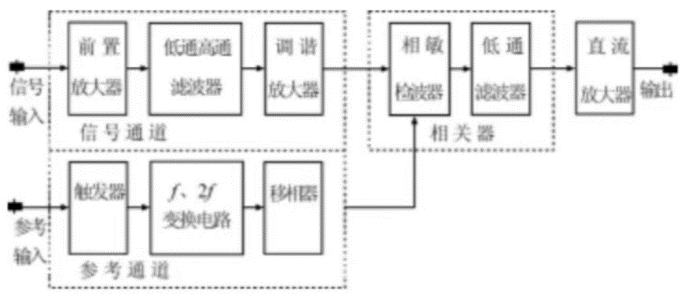
\includegraphics[width=.4\textwidth]{1.png}
	\caption{锁相放大器原理框图}	
	\label{LA}
\end{figure}
\subsection{锁相放大器的主要特征参量}
(1) 等效噪声带宽:锁相放大器采用 $RC$ 低通滤波器来作频带压缩,故其等效噪声带宽可类

比 $RC$ 低通滤波器,考虑到基波附近 $\pm \Delta f$ 的输入噪声都将在输出端产生噪声,故$\Delta f = \frac{1}{2RC}$。

对于白噪声,由于谐波响应应使锁相放大器总的等效噪声带宽为:
\begin{equation}
    \Delta f = \sum_{n=0}^{\infty} \frac{1}{(2n+1)^2} \frac{1}{2RC} = \frac{\pi^2}{16RC}
\end{equation}

减小带宽来抑制噪声是以牺牲响应速度为代价的,应选择适当的时间常数。

(2) 信噪比改善 ($SNIR$)。信噪比 ($SNR$) 是指系统输入信号幅度和噪声幅度之比,用$S/N$
来表示。信噪比改善是指系统输出端信噪比$S_o / N_o$ 与输入端信噪比$S_i / N_i$的比值,即:
\begin{equation}
    SNIR = \frac{S_o / N_o}{S_i / N_i}
\end{equation}

在白噪声的理想情况下,锁相放大器的信噪比改善在不计谐波响应时,表示为输入信号的噪
声带宽 $\Delta f_{ni}$ 与相干检测器输出噪声带宽之比 $\Delta f_{no}$ 的平方根表示,即:
\begin{equation}
    SNIR = \sqrt{\frac{\Delta f_{ni}}{\Delta f_{no}}}
\end{equation}

(3) 满刻度输出时的信号输入电平:表征了锁相放大器的测量灵敏度。

(4) 最大过载电平:即允许的最大非相干信号 (噪声) 的输入电平。

(5) 最小可分辨信号电平:由前置放大器输入端等效输入噪声和输出直流漂移$\delta$来决定。

(6) 输入总动态范围:定义为在给定测量灵敏度条件下锁相放大器的最大过载电平 $OVL$ 与
    最小可分辨信号 $MDS$ 之比的分贝值。

(7) 输出动态范围:满刻度输出时的输入电平 $FS$ 与最小可分辨信号 $MDS$ 之间的分贝值。

(8) 动态储备:锁相放大器的过载电平 $OVL$ 与满刻度输出时的输入电平 $FS$ 之比的分贝值。
\section{实验过程}
\subsection{实验仪器}
本实验的主要仪器是ND-501型微弱信号检测实验综合装置。实验线路图如下:
\begin{figure}[H]
	\centering
	
\includegraphics[width=.4\textwidth]{2.png}
	\caption{参考特性观测电路图}	
	\label{circuit1}
\end{figure}
\begin{figure}[H]
	\centering
	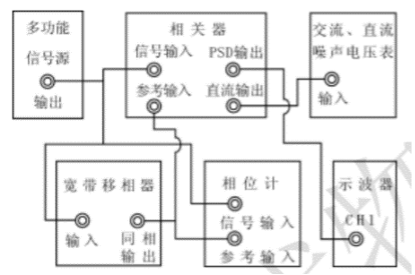
\includegraphics[width=.4\textwidth]{3.png}
	\caption{PSD输出波形观测电路图}
	\label{circuit2}
\end{figure}
\begin{figure}[H]
	\centering
	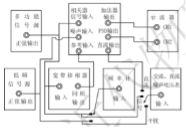
\includegraphics[width=.4\textwidth]{4.png}
	\caption{相关器对不相关信号的抑制电路图}
	\label{circuit3}
\end{figure}
\begin{figure}[H]
	\centering
	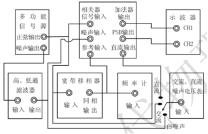
\includegraphics[width=.4\textwidth]{5.png}
	\caption{相关器对噪声的抑制电路图}
	\label{circuit4}
\end{figure}

\subsection{参考信号通道特性研究}
(1) 首先按照图 2 连接线路,用频率计测量输出信号频率,用交流直流噪声电压表测量信号的幅度,调节输出信号的频率为 $1kHz$ 左右,幅度大小为 $100mV$ 左右。

(2) 改变输入信号和参考信号之间的相位差,记录相位差为 $0^\circ$、$90^\circ$、$180^\circ$、$270^\circ$对应的宽带移相器的输入和输出信号的波形。

(3) 改变信号的幅值和频率,观察同相输出信号幅值和频率的变化,并做简要分析。

(4) 调节信号源,使输出波形分别为三角波和方波,重复上述观测。

\subsection{相敏检波器 PSD 输出波形和电压测量}
(1) 按照图 3 连接线路,置交流放大倍数为$\times1$,直流放大倍数为$\times10$,相关器低通滤波器时间常数置 1 秒。改变相位差,观察信号、参考信号及 PSD 的输出波形并分析它们的关系。

(2) 测量相关器输出直流电压大小与信号、参考信号之间幅值及相位差$\varphi$的关系。

(3) 用相位计测量$\varphi$值大小,记录参考信号和输入信号的相位差分别为 $0^\circ$、$90^\circ$、$180^\circ$、$270^\circ$时,PSD 输出直流信号$u_{dc}$和在示波器上的输出波形。

\subsection{相关器的谐波响应的测量与观察}
(1) 将图 3 中宽带带移相器的输入信号接至多功能信号源的“倍频•分频输出”,多功能信号源功能“选择”置“分频”,此时,参考信号的频率为信号频率的 $1/n$ 次倍。先置分频数为 1,调节移相器的相移量,使输出直流电压最大,记录输出直流电压的大小。

(2) 改变 n 的数值,重复上述测量,记录数据和图像并分析。

\subsection{相关器对不相关信号的抑制}
(1) 按照图 4 连接线路,选择相关器的交流放大倍数$\times1$,直流放大倍数$\times10$,时间常数 1 秒,调节多功能信号源的频率为 $200Hz$ 左右,电压为 $100mV$ 左右,先不加噪声,调节宽带带相移器的相移量,使相关器输出的直流电压最大,并测量其电压值。

(2) 加噪声并调节低频信号源的输出电压为 $300mv$,即干扰电压为待测量信号电压的 3 倍。从 $1200Hz$ 开始,逐步减小低频信号源频率,观测此时被测信号与干扰信号波形及相关器的输出直流电压变化 (重点关注频率接近输入信号的奇次谐波时的现象)。

\subsection{相关器对噪声的抑制及等效噪声带宽}
(1) 按图 5 连接线路,相关器选$K_{AC} = 10$, $K_{DC} = 10$, $T = 1$ 秒。输入信号频率$f_s = 1KHz$, $V_{si} = 50mV$。先不加白噪声,调节相移器的相移,使输入信号与参考信号同相,并用示波器观察“加法器输出”“PSD 输出”的波形,用电压表测量输出电压。

(2) 加白噪声信号,调节白噪声信号源的输出幅度或与高、低通滤波器的放大倍数相配合调节,使输入白噪声均方根电压为 $100mV$,计算输入信号的信噪比。用电压表测量相关器输出的信号电压和噪声电压,计算输出信号的信噪比,进而计算信噪比改善。


\section{实验结果的分析与讨论}

\subsection{参考信号通道特性研究}

(1) 控制信号源频率 $f = 1000.25Hz$ 不变, 改变信号源幅值, 观察同相输出信号的幅值变化

\begin{table}[H]
	\centering
	\caption{参考输出信号幅值与信号源幅值之间的关系}
	\begin{tabular}{ |c|c|c|c|c| } 
	 \hline
	 信号源幅值/mV & 98.9 & 151.7 & 356 & 1053 \\ 
	 \hline
	 参考输出幅值/mV & 5.017 & 5.017 & 5.017 & 5.017 \\ 
	 \hline
	\end{tabular}
\end{table}

分析: 由表1可得, 在控制信号源频率不变的情况下, 改变信号源信号的幅值, 参考输出信号的幅值不变, 这说明宽带移相器输出波的幅值与输入波幅值无关, 为固定值。

(2) 控制信号源幅值 $U = 99.5mV$ 不变, 改变信号源频率, 观察同相输出信号的频率变化

\begin{table}[H]
\centering
\caption{参考输出信号频率与信号源频率之间的关系}
\begin{tabular}{ |c|c|c|c|c| } 
 \hline
 信号源频率/Hz & 1000.39 & 1569.7 & 2125.5 & 5299.8 \\ 
 \hline
 参考输出频率/Hz & 1000.2 & 1574.0 & 2128.5 & 5275.5 \\ 
 \hline
\end{tabular}
\end{table}

分析: 由表2可知, 在误差允许范围内, 参考输出信号频率与信号源频率相等, 宽带移相器输出的参考信号频率可以由输入信号频率调控。

(3) 记录参考信号和信号源相位差分别为 $0^\circ$、 $90^\circ$、 $180^\circ$、 $270^\circ$ 时宽带移相器的输入和输出信号的波形。

\begin{figure}[H]
    \centering
    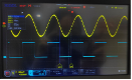
\includegraphics[width=.4\textwidth]{6.png}
    \label{example}
\end{figure}
\begin{figure}[H]
    \centering
    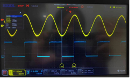
\includegraphics[width=.4\textwidth]{7.png}
    \label{example}
\end{figure}
\begin{figure}[H]
    \centering
    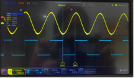
\includegraphics[width=.4\textwidth]{8.png}
    \label{example}
\end{figure}
\begin{figure}[H]
    \centering
    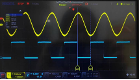
\includegraphics[width=.4\textwidth]{9.png}
    \caption{参考信号和信号源相位差分别为 0°、90°、180°、270°时宽带移相器的输入和输出信号的波形}	
    \label{example}
\end{figure}

分析:A. 观察输出波形,我们可以看到对于相位差为$0^\circ$时,方波突变点(正值突变为负值)对应正弦波零值;相位差为$90^\circ$时,方波突变点对应正弦波最小值;$180^\circ$时,方波突变点对应正弦波零值;$270^\circ$时,方波突变点对应正弦波最大值。

B. 改变参考信号和信号源的相位差,宽带移相器的输入(正弦波)和输出(方波)波形的相位差也随之进行相同变化,但不同相位差对应的输入和输出波的频率始终是相同的,这一图像规律也与上面得到的参考信号和信号源频率之间的关系一致。

C. 将正弦波换为方波或者三角波,输出波仍然为方波,且其规律与上述规律相同。

\subsection{相敏检波器 PSD 输出波形和电压测量}

(1) 输入信号、参考信号及 PSD 的输出波形之间的关系 (交流放大倍数$K_{AC}$=1):

\begin{figure}[H]
    \centering
    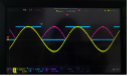
\includegraphics[width=.4\textwidth]{10.png}
    \label{example}
\end{figure}
\begin{figure}[H]
    \centering
    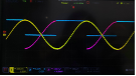
\includegraphics[width=.4\textwidth]{11.png}
    \label{example}
\end{figure}
\begin{figure}[H]
    \centering
    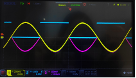
\includegraphics[width=.4\textwidth]{12.png}
    \label{example}
\end{figure}
\begin{figure}[H]
    \centering
    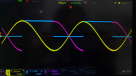
\includegraphics[width=.4\textwidth]{13.png}
    \caption{宽带移相器的相移量为 $0^\circ$、$90^\circ$、$180^\circ$、$270^\circ$时输入信号、参考信号及 PSD 输出信号的波形}	
    \label{example}
\end{figure}

分析:

A. 频率:参考信号与输入信号的频率相等且为 PSD 输出信号频率的两倍。

B. 幅度:在交流放大倍数$K_{AC}$=1 的情况下,PSD 输出信号的幅度=输入信号幅度$\times$与参考信号同频同相但幅度为 1 的方波。

C. 调节交流放大倍数$K_{AC}$=10,则 PSD 输出信号的幅度变为原来的十倍,频率不变;调节直流放大倍数$K_{DC}$=1,输入信号、参考信号、PSD 输出信号均不变。

(2) 探究相关器输出直流电压大小与信号、参考信号之间幅值及相位差$\varphi$的关系 (设置$K_{AC}$=1, $K_{DC}$=1)

\textbf{A. 控制输入信号幅值为$U = 209 mV$,探究直流电压大小与相位差$\varphi$的关系}

\begin{table}[H]
	\centering
	\caption{实验数据记录}
	\small
	\begin{tabular}{c|ccc}
		\Xhline{1.0pt}
		$\Delta \varphi$ & $0^\circ$ & $9.61^\circ$ & $16.1^\circ$ \\
		\Xhline{0.5pt}
		$V_{DC}$ & 2.11V & 2.07V & 2.00V \\
		\Xhline{0.5pt}
		$\Delta \varphi$ & $27.63^\circ$ & $33.44^\circ$ & $39.1^\circ$ \\
		\Xhline{0.5pt}
		$V_{DC}$ & 1.83V & 1.71V & 1.57V \\
		\Xhline{0.5pt}
		$\Delta \varphi$ & $47.2^\circ$ & $56.5^\circ$ & $65.11^\circ$ \\
		\Xhline{0.5pt}
		$V_{DC}$ & 1.37V & 1.09V & 0.81V \\
		\Xhline{0.5pt}
		$\Delta \varphi$ & $79.3^\circ$ & $92.9^\circ$ & $105.02^\circ$ \\
		\Xhline{0.5pt}
		$V_{DC}$ & 0.29V & -0.21V & -0.64V \\
		\Xhline{0.5pt}
		$\Delta \varphi$ & $117.41^\circ$ & $124.9^\circ$ & $137.0^\circ$ \\
		\Xhline{0.5pt}
		$V_{DC}$ & -1.05V & -1.30V & -1.63V \\
		\Xhline{0.5pt}
		$\Delta \varphi$ & $151.30^\circ$ & $175.8^\circ$ & $179.25^\circ$ \\
		\Xhline{0.5pt}
		$V_{DC}$ & -1.92V & -2.12V & -2.12V \\
		\Xhline{1.0pt}
	\end{tabular}
\end{table}

对数据进行基于最小二乘法的三角函数拟合,得到拟合函数为:
\begin{equation}
	V_{DC} = 2.12 \cdot \cos(\Delta \varphi - 2.51 \deg) - 0.01
\end{equation}
拟合结果如图\ref{fit}所示,拟合优度$R^2 = 0.9999$,表明拟合效果良好。
\begin{figure}[H]
	\centering
	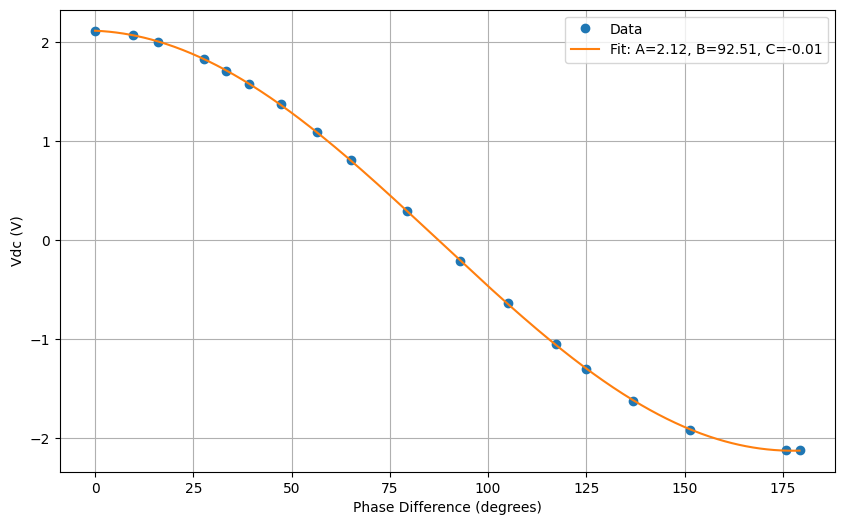
\includegraphics[width=.4\textwidth]{sin.png}
	\caption{相关器输出直流电压与相位差的关系}	
	\label{fit}
\end{figure}
分析:由图\ref{fit}可知,相关器输出直流电压$V_{DC}$与相位差$\Delta \varphi$之间呈余弦函数关系,且当相位差为$0^\circ$时,输出电压最大,幅值为$2.12V$。当相位差为$90^\circ$时,输出电压为$0V$;当相位差为$180^\circ$时,输出电压最小,幅值为$-2.12V$。
当相位差为$270^\circ$时,输出电压为$0V$。这说明相关器的输出电压与输入信号和参考信号之间的相位差$\varphi$有着密切的关系。

\textbf{B. 控制相位差$\varphi = 0^\circ$,探究直流电压大小与信号、参考信号之间幅值的关系}

\begin{table}[H]
    \centering
    \caption{相关器输出直流电压大小与信号幅值之间的关系}
    \begin{tabular}{c|cccc}
        \toprule
        $U_{dc}/\si{mV}$ & 57 & 110.9 & 175.3 & 269  \\
        \midrule
        信号幅值$/\si{mV}$ & 57.4 & 111.9 & 177.1 & 268  \\
		\midrule
		$U_{dc}/\si{mV}$ & 396 & 504 & 824 & \\
        \midrule
        信号幅值$/\si{mV}$  & 396 & 504 & 828 & \\
        \bottomrule
    \end{tabular}
	\label{table:dc}
\end{table}

图像拟合:

\begin{figure}[H]
    \centering
    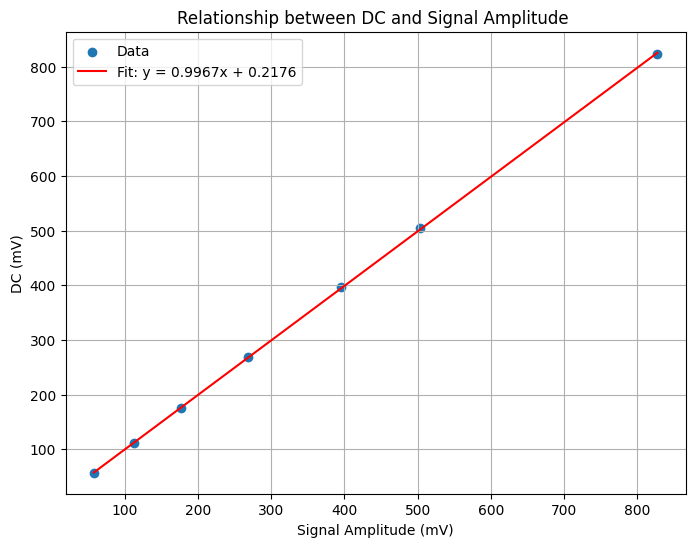
\includegraphics[width=0.4\textwidth]{phi0.png}
    \caption{相关器输出直流电压大小与信号幅值之间的关系图}
	\label{fig:input}
\end{figure}

分析:由表 \ref{table:dc} 和图 \ref{fig:input} 可得,拟合得出 $u_{dc} = 0.9967u - 0.2176$。在误差允许范围内,相关器输出直流电压大小与信号幅值成正比关系,满足公式 (4)。



\printbibliography
\end{multicols}

\end{document}
